\documentclass[3p,times,procedia]{elsarticle}
\flushbottom

\usepackage{ecrc}
\usepackage{graphicx}

\usepackage{caption}
\usepackage{subcaption}
\makeatletter
\def\black{\special{color cmyk 0 0 0 1.0}}
\def\blue{\special{color rgb 0 0.502 0.675}}
\def\url#1{\special{color push}{\special{color push}\blue#1\special{color pop}}\special{color pop}\black}
\makeatother

\volume{00}
\firstpage{1}
\journalname{Energy Procedia}
\runauth{E. Fonn et al.}
\jid{egypro}

\usepackage{amsmath}
\usepackage{amssymb}

\biboptions{sort&compress}

\usepackage{siunitx}
\usepackage[colorlinks=true, linkcolor=black, citecolor=black, urlcolor=black]{hyperref}
\usepackage{bm}
\usepackage{tikz}
\usetikzlibrary{shapes.geometric, positioning}

\begin{document}

\begin{frontmatter}

\dochead{12th Deep Sea Offshore Wind R\&D Conference, EERA DeepWind'2015}
\title{Spline based mesh generator for high fidelity simulation of flow around turbine blades}

\author[a]{E. Fonn \corref{cor1}}
\author[a]{A. Rasheed}
\author[a]{A. M. Kvarving}
\author[a,b]{T. Kvamsdal}
\address[a]{Applied Mathematics, SINTEF ICT, Trondheim 7035, Norway}
\address[b]{Mathematical Sciences, Alfred Getz vei 1, Trondheim 7091, Norway}

\begin{abstract}
  Mesh generation involving complex geometries, such as wind turbine blades, is
  highly complicated. The problem is generally addressed using tetrahedral meshes,
  or hybrid meshes with hexahedral elements close to the body and tetrahedral
  elements elsewhere. The popularity of such mesh generators can be attributed to
  their associated ease of use and relative eutomation, which comes at the cost of
  numerical accuracy in the subsequent analysis. Added to this, such meshes can
  generally not represent the true geometry. Isogeometric analysis (IGA), offering
  an integration of analsis and CAD geometry through use of the same basis
  functions, has been catching up since 2005. The method offers demonstrably
  better accuracy, as well as an exact geometric representation. Since its
  inception, the method has been applied to problems from both fluid and
  structural mechanics. The availability of NURBS-based surface modeling software
  such as Rhinoceros has made it possible to create complex geometries with
  relative ease, but the lack of a volumetric spline-based mesh generator proves a
  bottleneck. In this paper we describe a mesh generator that has been developed
  at the Applied Mathematics Department of SINTEF ICT which can generate spline
  based block structured meshes of high quality for subsequent fluid or
  structural simulations.
\end{abstract}

\begin{keyword}
  Mesh generation \sep
  Wind turbine blades \sep
  Computational fluid dynamics \sep
  Variable turbulent intensity
\end{keyword}

\cortext[cor1]{Corresponding author. Tel.: +47-41449889}

\end{frontmatter}

\email{
  eivind.fonn@sintef.no,
  adil.rasheed@sintef.no,
  arne.morten.kvarving@sintef.no,
  trond.kvamsdal@sintef.no
}

\section{Introduction}

This work presents an automatic block-structured spline-based mesh generator for
wind turbine blades being developed to streamline the workflow from CAD modeling
to simulation and analysis. It was developed initially for the NREL 5MW
reference blade, but with a modular approach that will allow it to handle other
geometries as well.

The whole procedure can be subdivided into two steps: solid modeling or blade
construction and volumetric mesh generation. The mesh generation is performed
using cubic splines everywhere, and the spline order is then adjusted in the
final step before output, to also allow the creation of linear or quadratic
models.

\section{Methodology}

\subsection{Trailing edge modification of airfoils}

The NREL 5MW reference blade \cite{Jonkman2009drw} is defined in terms of
cross-sectional data at 19 points along the blade axis from $\SI{2}{m}$ to
$\SI{62.9}{m}$. At each point is defined the airfoil shape (in terms of an
ordered point cloud), the chord length (an isotropic scaling factor), the
aerodynamic center and the twist angle. The innermost airfoils (until about
$\SI{10}{m}$) are cylindrical, the middle (until about $\SI{40}{m}$) are Delft
University airfoils of various kinds, and the remaining cross sections are
NACA64 airfoils. See \autoref{fig:airfoils:note}.

Each airfoil is defined as a sequence of points
\[ \bm{x}_i = (x_i, f(x_i)) \pm \bm{n}_i t_i, \] where $0 \le x_i \le 1$ is the
chordlength parametrization, and $f$ is a function defining the shape of the
central line, on which the vector $\bm{n}$ is always normal. The numbers $t_i$
then give half the thickness of the airfoil at each point.

\begin{figure}
  \centering
  \begin{subfigure}[b]{0.45\textwidth}
    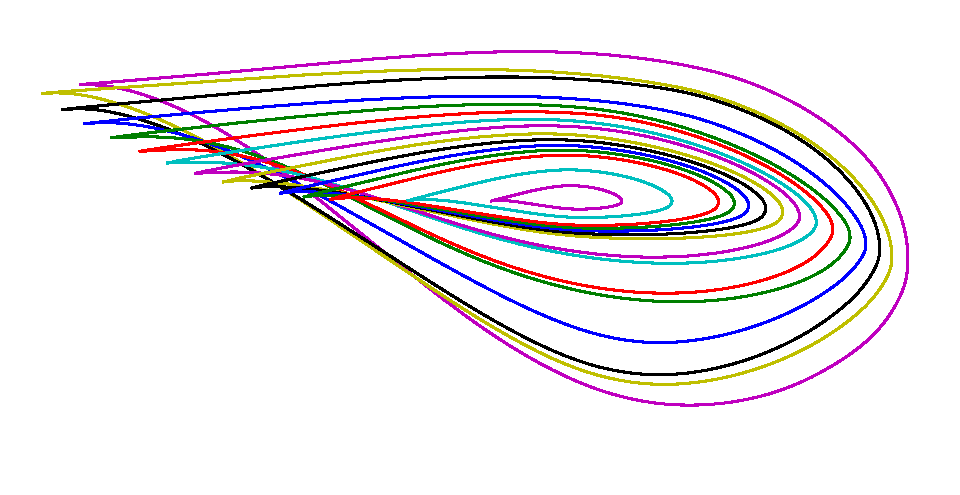
\includegraphics[width=\textwidth]{figs/airfoils-note}
    \caption{Sharp trailing edge}
    \label{fig:airfoils:note}
  \end{subfigure}
  \begin{subfigure}[b]{0.45\textwidth}
    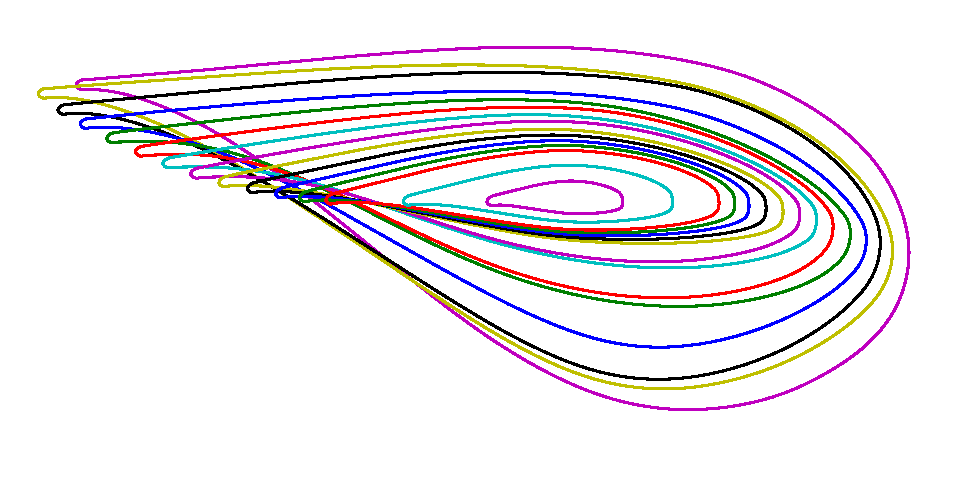
\includegraphics[width=\textwidth]{figs/airfoils-te}
    \caption{Trailing edge modification (exaggerated)}
    \label{fig:airfoils:te}
  \end{subfigure}
  \caption{Airfoils for the NREL 5MW wind turbine blade.}
\end{figure}

The defining characteristic of the airfoils is a sharp trailing edge. Typically,
this forces the construction of a ``C-mesh'' (\autoref{fig:cmesh}) with a large
waste of degrees of freedom in regions where they are not required (above and
below the trailing edge). In order to create a more efficient ``O-mesh'', we
introduce a modification to produce rounded trailing edges, as seen in
\autoref{fig:airfoils:te}. This is realized as a modification to the thickness
values, $\tilde{t}_i = t_i + \delta x_i$ will produce a trailing edge gap of
width $\delta$. A semicircle is then fitted in this gap with the required
continuity to complete the modified airfoil.

Typically the trailing edge is chosen to be of uniform physical size,
independent of the chord length, which means in practice that, for some airfoil
with chord length $c$, the unscaled gap width $\delta$ must be chosen as
$\delta(c) = \delta_0/c$. We have found small (around $\SI{1}{cm}$)
modifications to have negligible effect on observables (drag and lift). This
corresponds to a modification that is between $\SI{0.22}{\percent}$ and
$\SI{1.4}{\percent}$ of chord length. \autoref{fig:airfoils:te} shows the effect
exaggerated by a factor five.

\begin{figure}
  \centering
  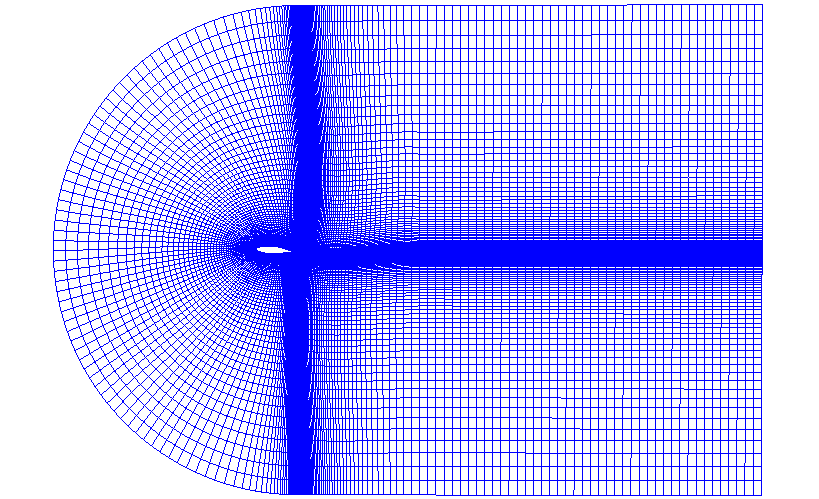
\includegraphics[width=0.4\textwidth]{figs/Sec41_a8_mesh}
  \caption{A ``C-mesh.''}
  \label{fig:cmesh}
\end{figure}

\subsection{Lengthwise interpolation}

It is desirable to use a higher resolution in the length direction than that
provided by the NREL 5MW specification. Cubic interpolation with suitable
boundary conditions can be used for this, but some care will have to be taken in
the intersection between DU airfoils and cylindrical cross sections. Because of
the sharp transition, a high order interpolator will cause the geometry to
self-intersect. This is fixed by an intermediate linear interpolation step
centered at the offending airfoil. See \autoref{fig:length-joined}.

\begin{figure}
  \centering
  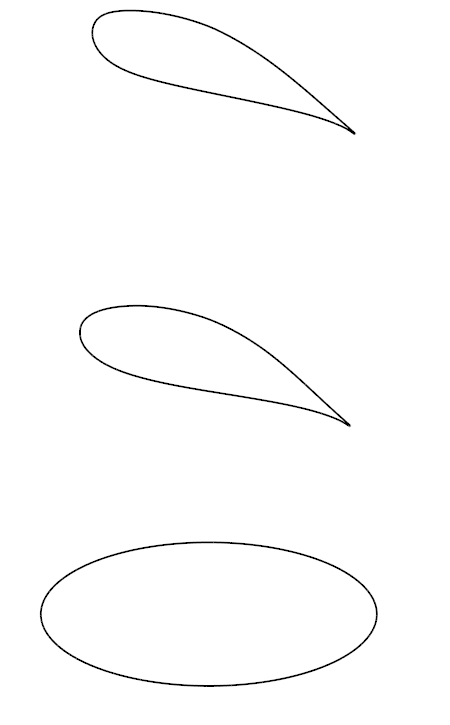
\includegraphics[width=0.2\textwidth]{figs/length-none}
  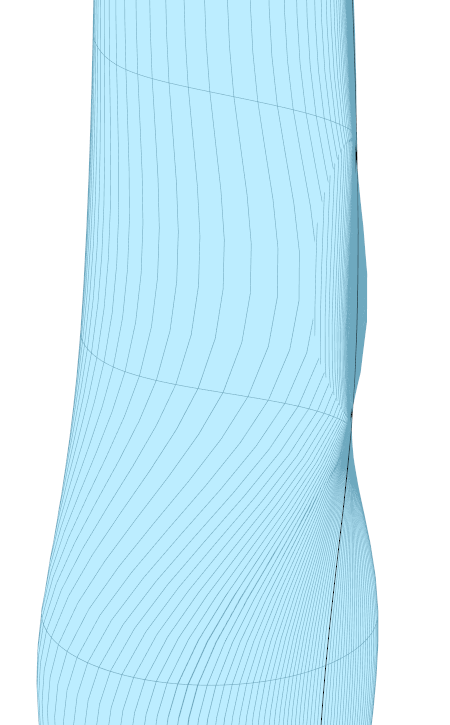
\includegraphics[width=0.2\textwidth]{figs/length-none-surf}
  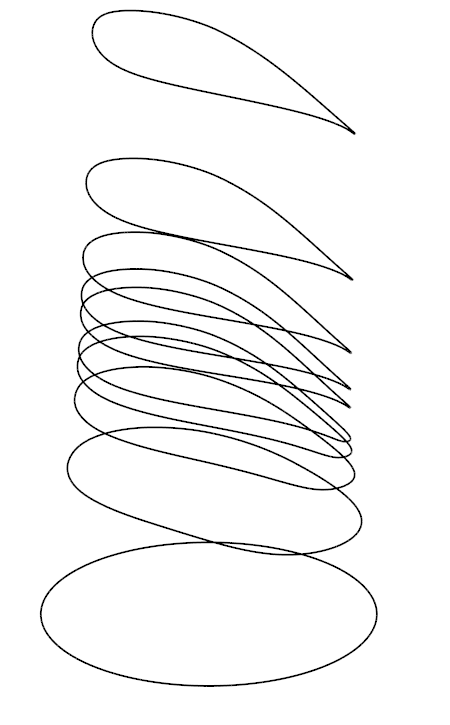
\includegraphics[width=0.2\textwidth]{figs/length-joined}
  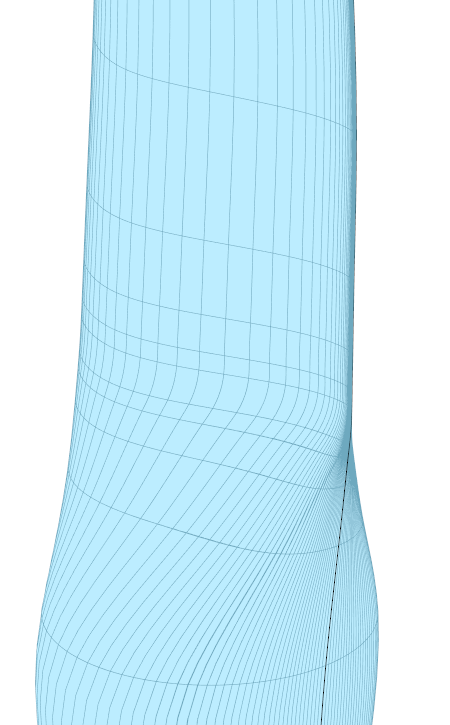
\includegraphics[width=0.2\textwidth]{figs/length-joined-surf}
  \caption{An intermediate interpolation step of lower order produces a
    non-self-intersecting mesh.}
  \label{fig:length-joined}
\end{figure}

\subsection{Transfinite interpolation}
\label{sec:tfi}

The basic premise of this section can be summarized in \autoref{fig:tfi}.

\begin{enumerate}
\item A circle is drawn around the aerodynamic center of each airfoil at a suitable radius.
\item The ``O-mesh'' is generated and then split into eight equal patches. \label{item:tfi-1}
\item The boundaries for eight additional patches is drawn, which creates a square mesh enveloping
  the ``O-mesh''.
\item The enclosed area is then meshed. \label{item:tfi-2}
\item Additional patches can then be fit to the outside as required.
\end{enumerate}

This method relies on a technique to mesh an area enclosed by four curves, as in
steps \ref{item:tfi-1} and \ref{item:tfi-2}. This method is \emph{transfinite
interpolation} (TFI), also known as the Gordon Hall algorithm
\cite{Gordon1973ccc}. The remainder of this section will deal with this
technique, its limitations, and how they are overcome.

\begin{figure}
  \centering
  \begin{subfigure}[b]{0.4\textwidth}
    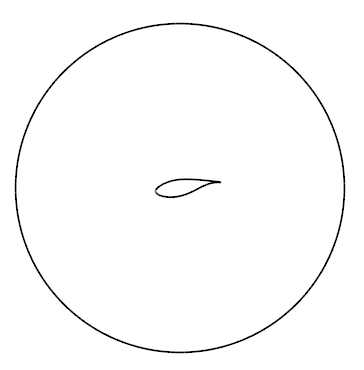
\includegraphics[width=\textwidth]{figs/tfi-1}
    \caption{Airfoil and circle.}
    \label{fig:tfi:1}
  \end{subfigure}
  \begin{subfigure}[b]{0.4\textwidth}
    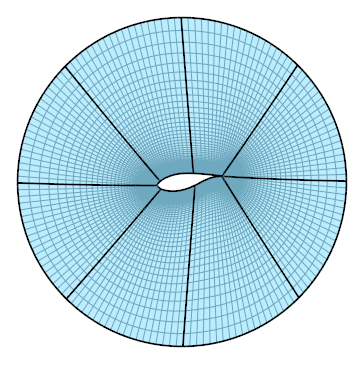
\includegraphics[width=\textwidth]{figs/tfi-2}
    \caption{``O-mesh'' filled in and split.}
    \label{fig:tfi:2}
  \end{subfigure}
  \\ \vspace{0.4cm}
  \begin{subfigure}[b]{0.4\textwidth}
    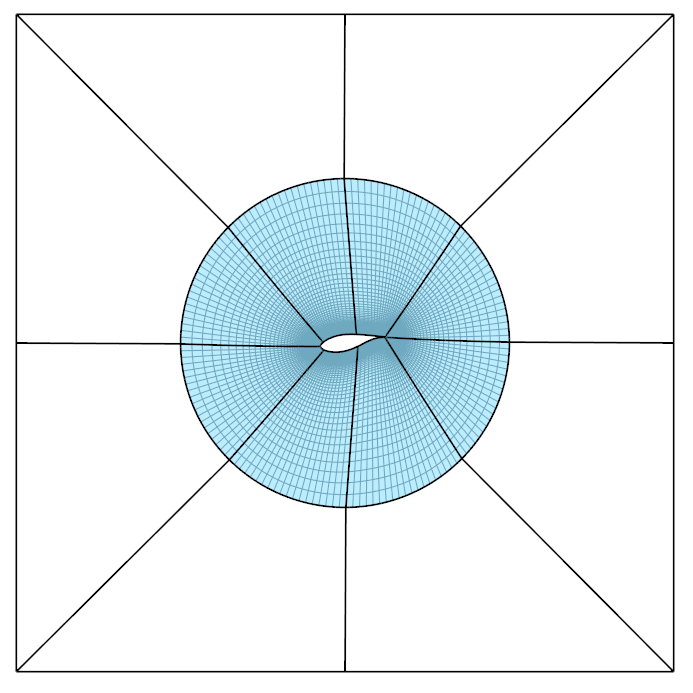
\includegraphics[width=\textwidth]{figs/tfi-3}
    \caption{``O-mesh'' and square.}
    \label{fig:tfi:3}
  \end{subfigure}
  \begin{subfigure}[b]{0.4\textwidth}
    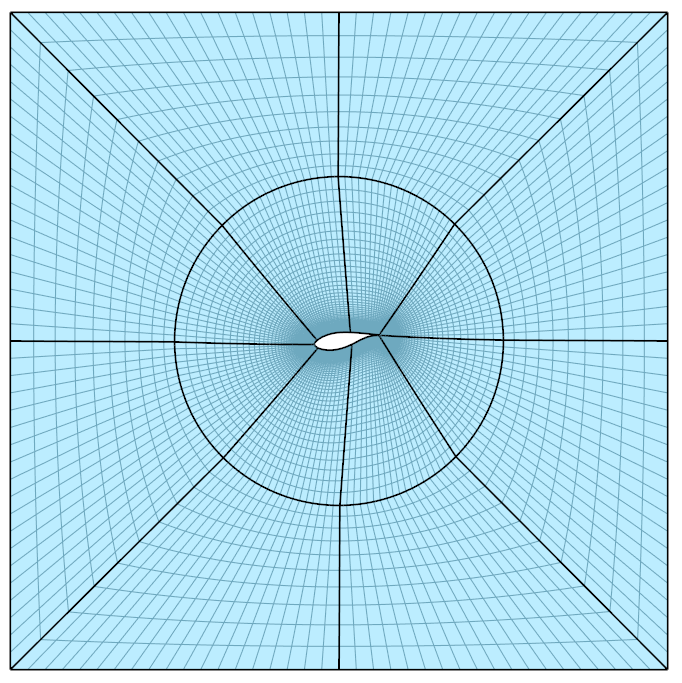
\includegraphics[width=\textwidth]{figs/tfi-4}
    \caption{Square filled in.}
    \label{fig:tfi:4}
  \end{subfigure}
  \\ \vspace{0.4cm}
  \begin{subfigure}[b]{0.7\textwidth}
    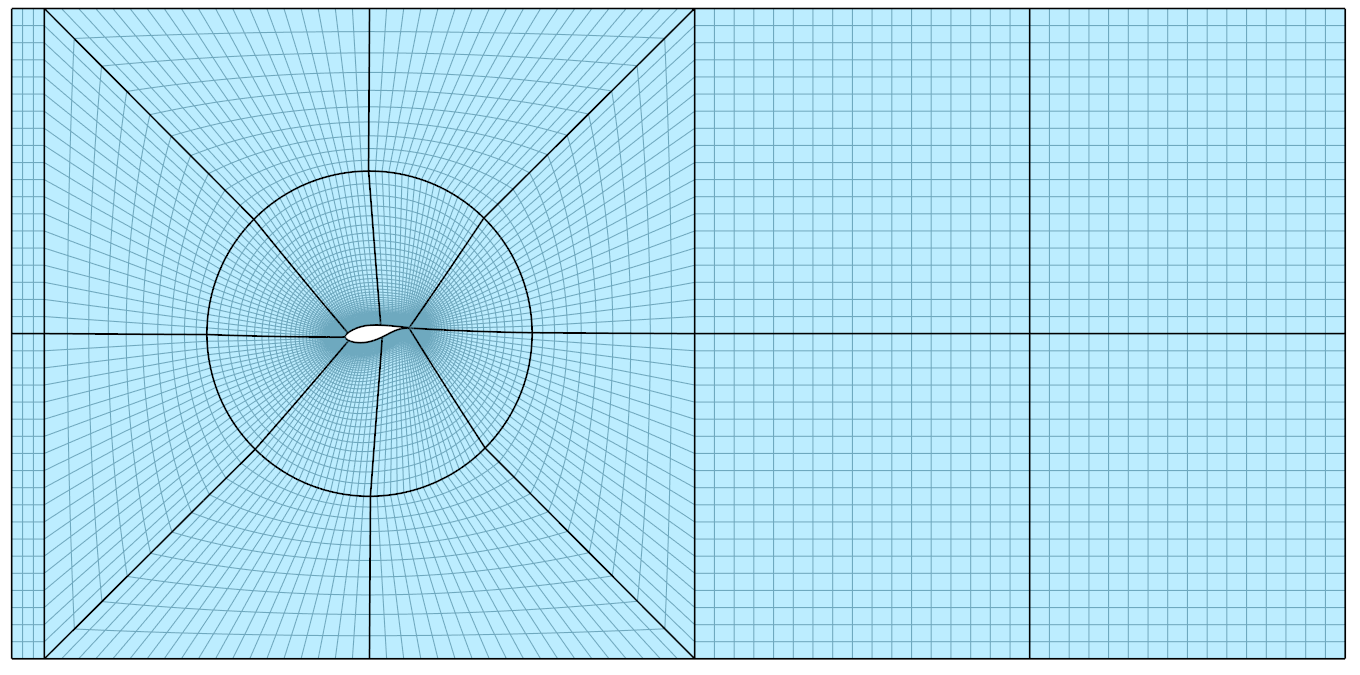
\includegraphics[width=\textwidth]{figs/tfi-5}
    \caption{Example of additional patches.}
    \label{fig:tfi:5}
  \end{subfigure}
  \caption{Strategy for two-dimensional mesh generation.  Compare with \autoref{fig:cmesh}.}
  \label{fig:tfi}
\end{figure}

\subsubsection{Linear TFI}

\begin{figure}
  \centering
  \begin{subfigure}[b]{0.4\textwidth}
    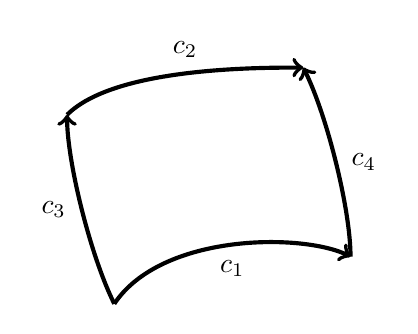
\begin{tikzpicture}[scale=3]
      \draw [->, line width=1.5pt] (0,0) .. controls (0.2, 0.3) and (0.8, 0.3) .. (1, 0.2)
      node[midway, below, inner sep=5pt] {$c_1$};
      \draw [->, line width=1.5pt] (0,0) .. controls (-0.1, 0.2) and (-0.2, 0.6) .. (-0.2, 0.8)
      node[midway, left, inner sep=5pt] {$c_3$};
      \draw [->, line width=1.5pt] (-0.2,0.8) .. controls (0, 1.0) and (0.6, 1.0) .. (0.8, 1.0)
      node[midway, above, inner sep=5pt] {$c_2$};
      \draw [->, line width=1.5pt] (1,0.2) .. controls (1.0, 0.4) and (0.9, 0.8) .. (0.8, 1.0)
      node[midway, right, inner sep=5pt] {$c_4$};
    \end{tikzpicture}
    \caption{Curve-to-surface TFI.}
    \label{fig:tfi-curves}
  \end{subfigure}
  \begin{subfigure}[b]{0.4\textwidth}
    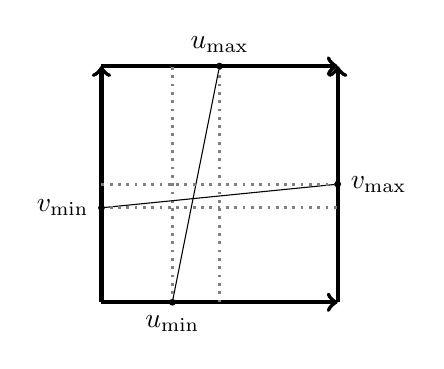
\begin{tikzpicture}[scale=3]
      \draw[->, line width=1.5pt] (0,0) -- (1,0);
      \draw[->, line width=1.5pt] (0,1) -- (1,1);
      \draw[->, line width=1.5pt] (0,0) -- (0,1);
      \draw[->, line width=1.5pt] (1,0) -- (1,1);
      \draw (0.3,0) -- (0.5,1);
      \draw[dotted, gray, line width=1pt] (0.3,0) -- (0.3,1);
      \draw[dotted, gray, line width=1pt] (0.5,0) -- (0.5,1);
      \draw (0,0.4) -- (1,0.5);
      \draw[dotted, gray, line width=1pt] (0,0.4) -- (1,0.4);
      \draw[dotted, gray, line width=1pt] (0,0.5) -- (1,0.5);
      \node [label=below:$u_\text{min}$, draw, fill=black, circle, inner sep=0pt, minimum size=2] at (0.3,0) {};
      \node [label=above:$u_\text{max}$, draw, fill=black, circle, inner sep=0pt, minimum size=2] at (0.5,1) {};
      \node [label=left:$v_\text{min}$, draw, fill=black, circle, inner sep=0pt, minimum size=2] at (0,0.4) {};
      \node [label=right:$v_\text{max}$, draw, fill=black, circle, inner sep=0pt, minimum size=2] at (1,0.5) {};
    \end{tikzpicture}
    \caption{Normalized TFI.}
    \label{fig:tfi-normalized}
  \end{subfigure}
\end{figure}

Given four curves parametrized as shown in \autoref{fig:tfi-curves}, the
enveloped area can be parametrized as follows, assuming without loss of
generality that the parameter domains of all curves are $[0,1]$.
\begin{align}
  \nonumber S(u,v) &= (1-v)c_1(u) + v c_2(u) + (1-u)c_3(v) + u c_4(v) \\
  \label{eqn:std-tfi} &- \left[(1-u)(1-v)c_1(0) + u(1-v)c_1(1)
                        + (1-u)v c_2(0) + u v c_2(1) \right]
\end{align}
This is essentially the sum of two linear interpolations (one in each direction)
minus the linear interpolation in both directions.

This simple method produces generally excellent and reliable results, with a few
exceptions.
\begin{itemize}
\item It is highly sensitive to the parametrization (not just the geometry) of
  the four curves.
\item It cannot guarantee orthogonal meshlines near the body, which is of
  interest in high Reynolds number CFD applications.
\item The Jacobian is not guaranteed to be everywhere positive, which means
  gridlines might intersect. This happens in rare cases of nonconvex domains.
\end{itemize}
In the following, we offer solutions to these problems.

\subsubsection{Normalized TFI}

It is sometimes useful to be able to produce distinct parametrizations of the
interior domain from distinct parametrizations of the surrounding curves, but in
our work we have found it useful to implement a parameter-normalized form of
TFI.

If all curves $c_i$ are parametrized by arclength, \eqref{eqn:std-tfi} produces
resonable results. However, since two opposing curves must have the same
parametrization, it is not generally possible for both to be simultaneously
parametrized by arclength.

Given parameters $u_\text{min}, u_\text{max}, v_\text{min}, v_\text{max}$ of
$c_1,\ldots, c_4$ respectively, corresponding for example to knots, the
normalized parameters of the interior should satisfy the following condition
(see \autoref{fig:tfi-normalized}),
\[
  u = u_\text{min} + v\underbrace{(u_\text{max} - u_\text{min})}_{\Delta u}, \qquad
  v = v_\text{min} + u\underbrace{(v_\text{max} - v_\text{min})}_{\Delta v}
\]
Whence we find the values $u, v$ for use in \eqref{eqn:std-tfi},
\begin{align*}
  \begin{pmatrix} u \\ v \end{pmatrix} =
  \frac{1}{1-\Delta u\Delta v}
  \begin{pmatrix} 1 & \Delta u \\ \Delta v & 1 \end{pmatrix}
  \begin{pmatrix} u_\text{min} \\ v_\text{min} \end{pmatrix}.
\end{align*}

\subsubsection{Orthogonalized TFI}

To obtain orthogonal meshlines near the airfoil (\autoref{fig:orthogonal}), we
employ an algorithm that grows the mesh layer by layer from the body outwards.
At each step $j$, the gridpoints on the next layer are given by a weighted mean,
\begin{equation} \label{eqn:blending}
  \bm{p}^j_i = \alpha_j \bm{q}^j_i + (1 - \alpha_j) \bm{t}^j_i.
\end{equation}
Here, $\bm{t}$ denotes the points produced by \eqref{eqn:std-tfi}, and $\bm{q}$
denotes the orthogonally projected points from the previous layer, i.e.
\[
  \bm{q}^j_i = \bm{p}^{j-1}_i + \bm{n}^{j-1}_i \Delta^j_i
\]
where $\bm{n}$ denotes the normal to each layer curve and $\Delta^j_i$ is a
suitable distance function.

The coefficient $\alpha_j$ controls the orthogonality of the mesh at each step,
and should vanish as $j$ grows. A suitable choice is
\[
  \alpha_j = \begin{cases}
    1, & j \leq k, \\
    0, & j = N, \\
    r_\alpha^{j-k}, & \text{otherwise.}
  \end{cases}
\]
where $k$ is the number of elements in the boundary layer, $N$ is the total
number of elements and $r_\alpha < 1$.

\begin{figure}
  \centering
  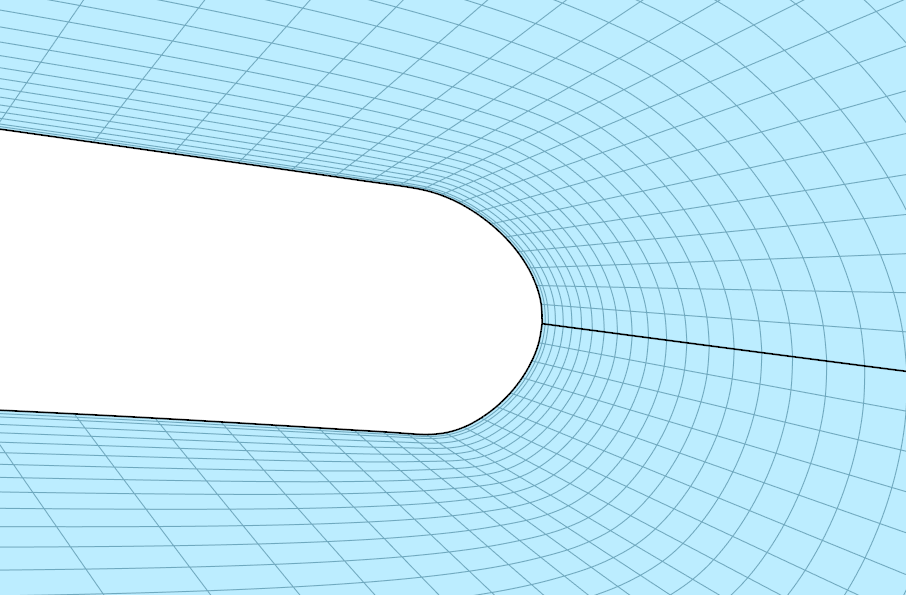
\includegraphics[width=0.4\textwidth]{figs/nonorthogonal}
  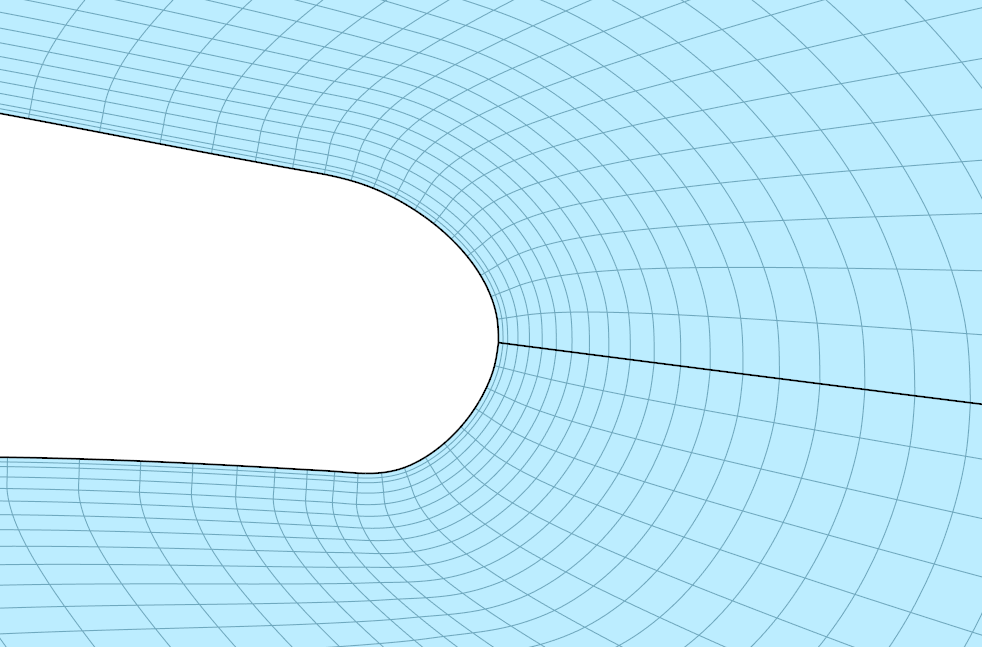
\includegraphics[width=0.4\textwidth]{figs/orthogonal}
  \caption{Orthogonal meshlines near the trailing edge.}
  \label{fig:orthogonal}
\end{figure}

\subsection{Smoothed TFI}

The given algorithm may produce negative-Jacobian meshes in some cases,
particularly for concave geometries and, in connection with orthogonality, large
boundary layers. To combat this, one may perform a Laplacian smoothing on the
orthogonally projected points $\bm{q}$ prior to \eqref{eqn:blending}. If the
precise distribution of the final layer points is not critical, it might be more
effective to perform the smoothing \emph{after} \eqref{eqn:blending}, on the
points $\bm{p}$. Note that this smoothing operator should act on the parameter
space of the curve traced out by the points rather than on the points directly.
The smoothing factor should behave much like $\alpha$, possibly with a larger
decay factor. See \autoref{fig:laplacian}.

\begin{figure}
  \centering
  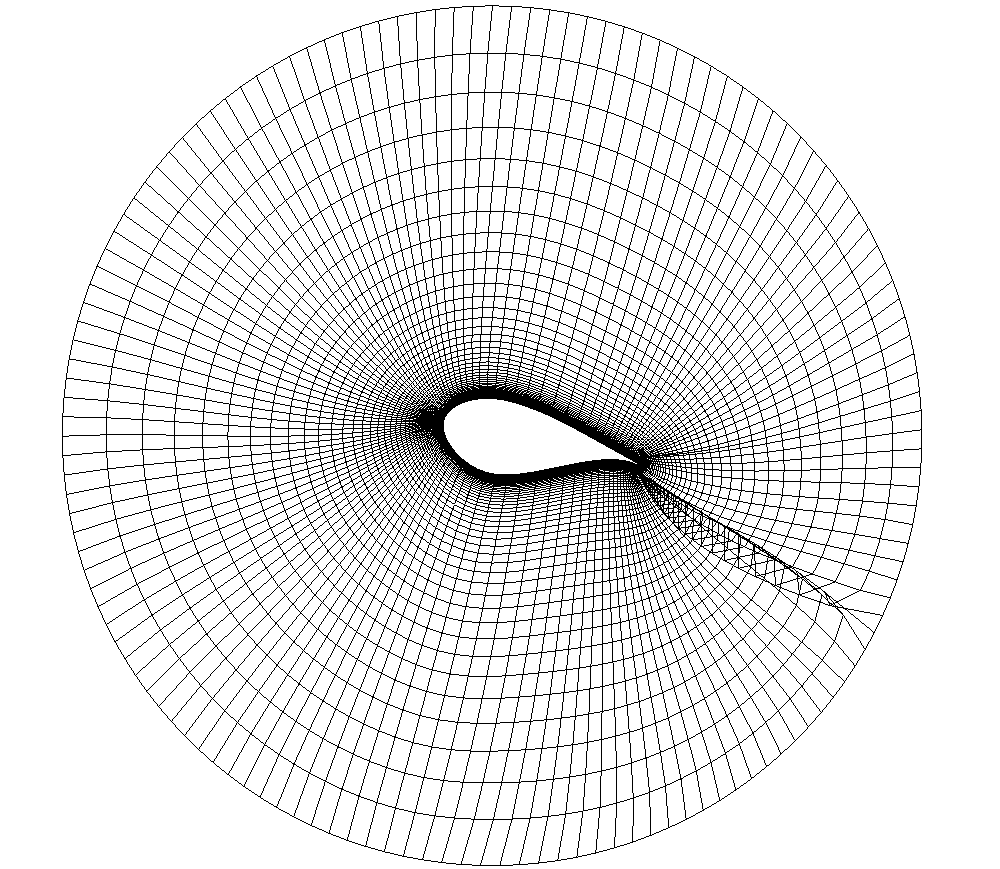
\includegraphics[width=0.35\textwidth]{figs/section12}
  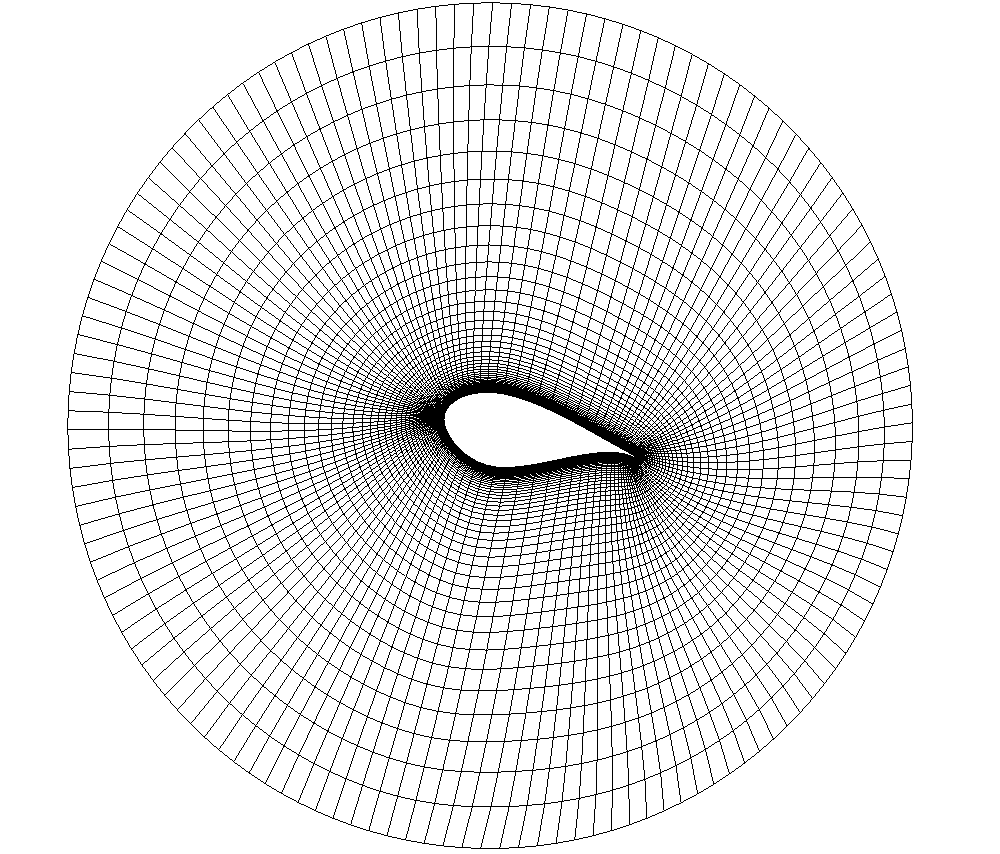
\includegraphics[width=0.35\textwidth]{figs/section12_smooth}
  \caption{Laplacian smoothing.}
  \label{fig:laplacian}
\end{figure}

\subsection{Tip geometry and closure}

We here describe a heuristic algorithm for generating a closed tip geometry,
which is fitted on the final airfoil in a $C^1$-continuous manner. To form the
basic geometry of the tip, we construct the midpoint of the final airfoil, and
raise it a suitable distance (here, about $\SI{20}{cm}$) to produce a center
point. We then interpolate between the two endpoints of the airfoil and the
center point to produce a raised midline. At each pair of corresponding points
on the airfoil, we can now interpolate to form a cross-curve orthogonal to the
raised midline. This produces a parametrization of the tip geometry, with
singularities. This geometry can then be partitioned into twelve non-singular
patches as shown in \autoref{fig:tip-geometry}.

For the eight patches not touching the singular points of the original
para-metrization, this is most easily done by constructing a mesh on the
parameter domain and mapping it accordingly. For the other four patches, we have
performed ordinary TFI in physical space as already described. The resulting
geometry can then be projected by least distance onto the wingtip.

\begin{figure}
  \centering
    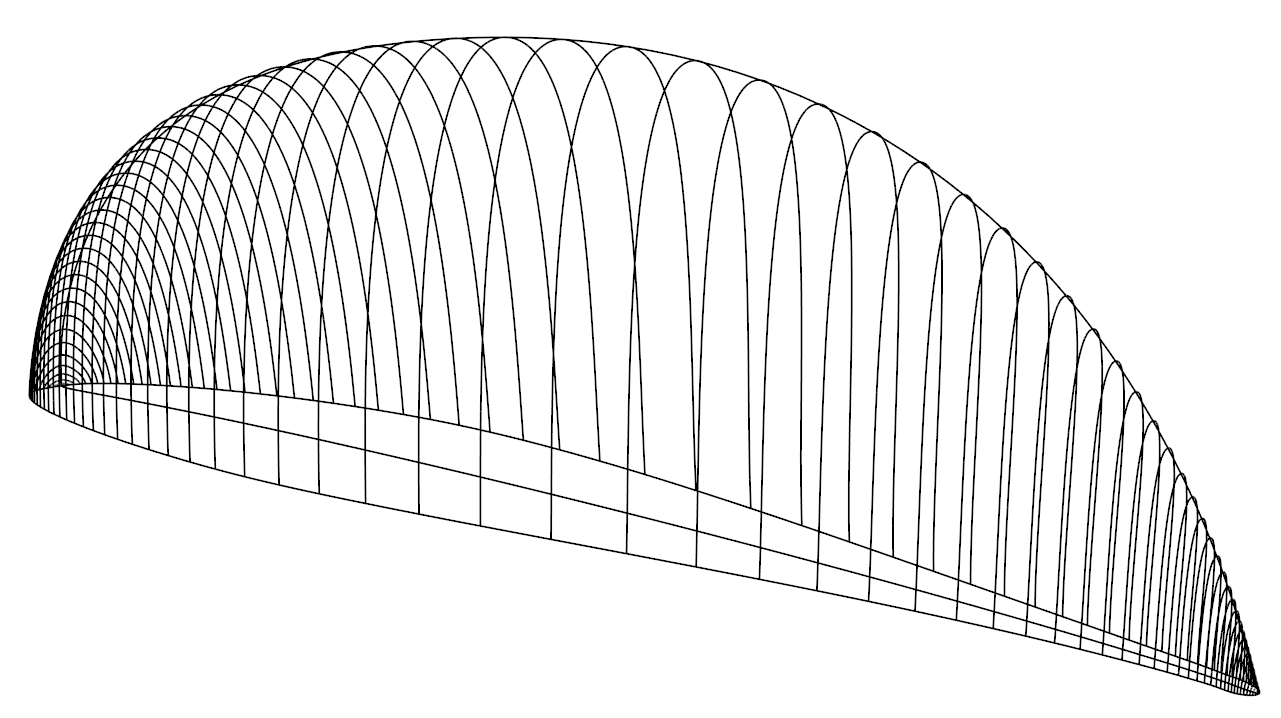
\includegraphics[width=0.4\textwidth]{figs/wingtip-skeleton}
    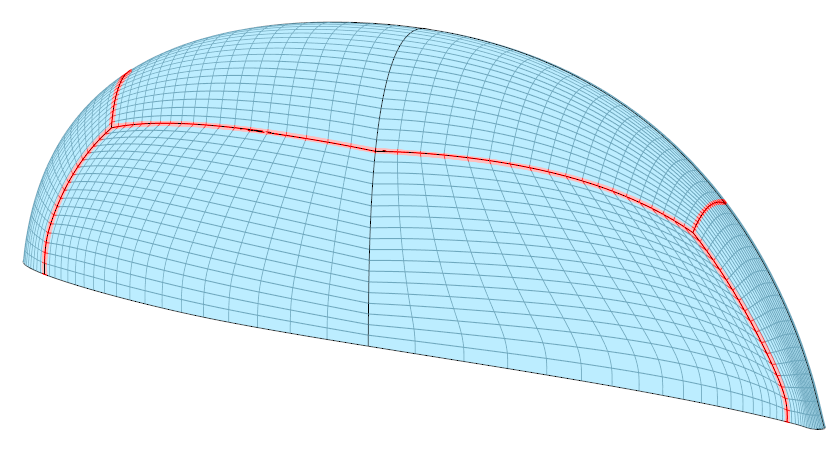
\includegraphics[width=0.4\textwidth]{figs/wingtip-full}
    \caption{Constructing the tip geometry.}
    \label{fig:tip-geometry}
\end{figure}

\subsection{Surrounding mesh}

To produce the surrounding volumetric wingtip mesh, we rely on volumetric TFI,
which can be used to mesh the volume enclosed in six surfaces, and to which all
the modifications described in \autoref{sec:tfi} carry over in more or less
straightforward manner.

The strategy is then:
\begin{enumerate}
\item Form the curves describing the patch structure of the surrounding mesh.
\item Form the surfaces between these curves using two-dimensional
  TFI. \label{item:vol-tfi-surf}
\item Form the volumes using volumetric TFI.
\end{enumerate}

Most of the surfaces required in step \ref{item:vol-tfi-surf} can be generated
immediately using the same algorithm as already described. The remainder require
the formation of four central curves emanating from the center point of each
quadrant. This can be done by ordinary interpolation, but a better method is to
combine two patch curves emanating from the center point (marked with red in
\autoref{fig:tip-geometry}) as a spline curve with a $C^0$ discontinuity,
perform TFI with the corresponding outer curve, and extracting the necessary
curve from the resulting surface. This allows the remaining surfaces to be
generated. See \autoref{fig:flower}.

\begin{figure}
  \centering
  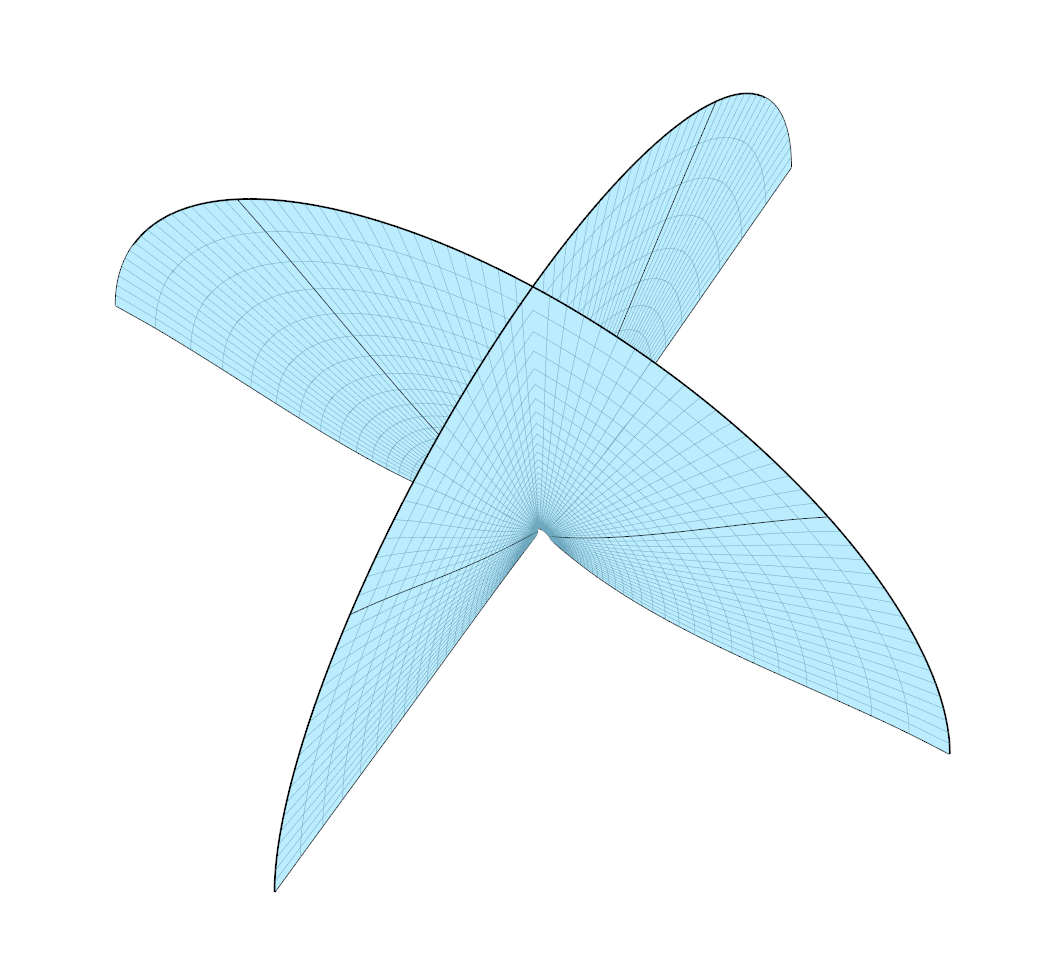
\includegraphics[width=0.3\textwidth]{figs/wingtip-first}
  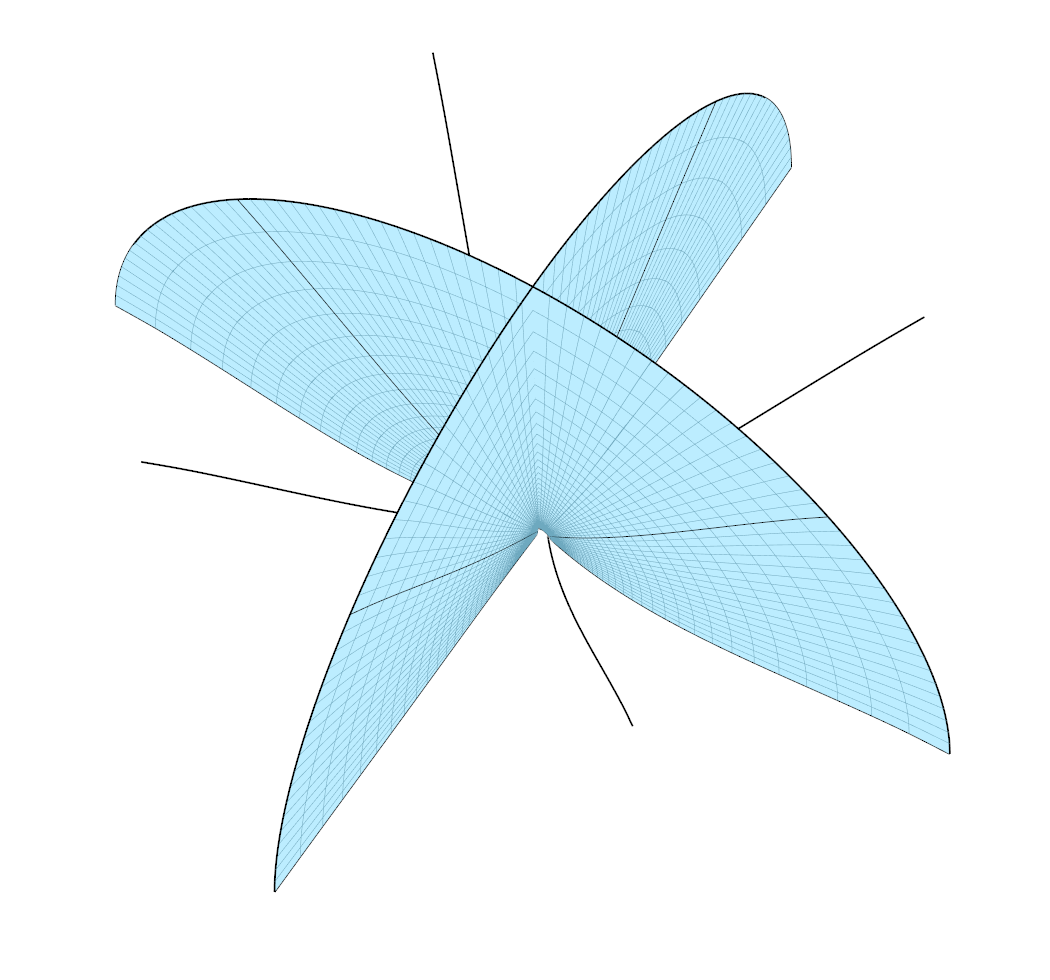
\includegraphics[width=0.3\textwidth]{figs/wingtip-centers}
  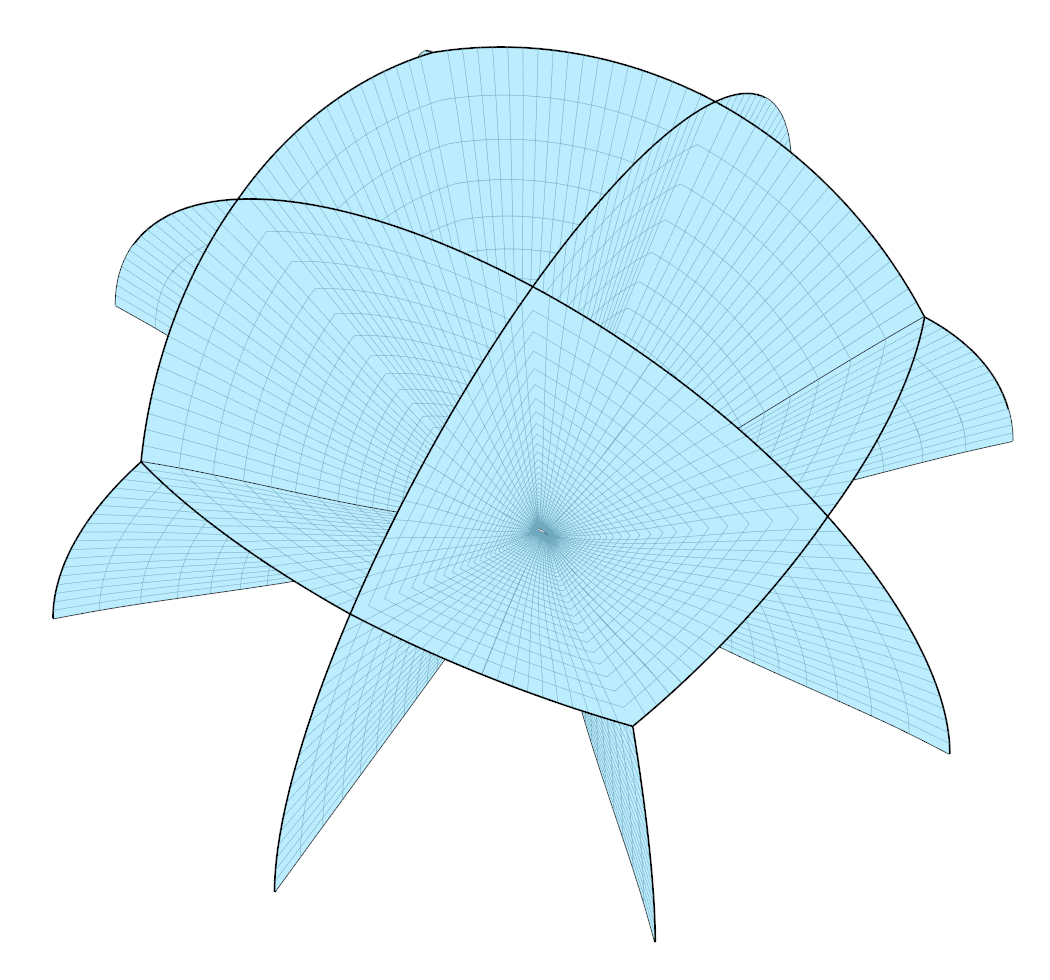
\includegraphics[width=0.3\textwidth]{figs/wingtip-flower}
  \caption{Generating the surfaces of the surrounding mesh.}
  \label{fig:flower}
\end{figure}

The block structure of the completed mesh, with four radial patches, can be seen
in \autoref{fig:full}.

\begin{figure}
  \centering
  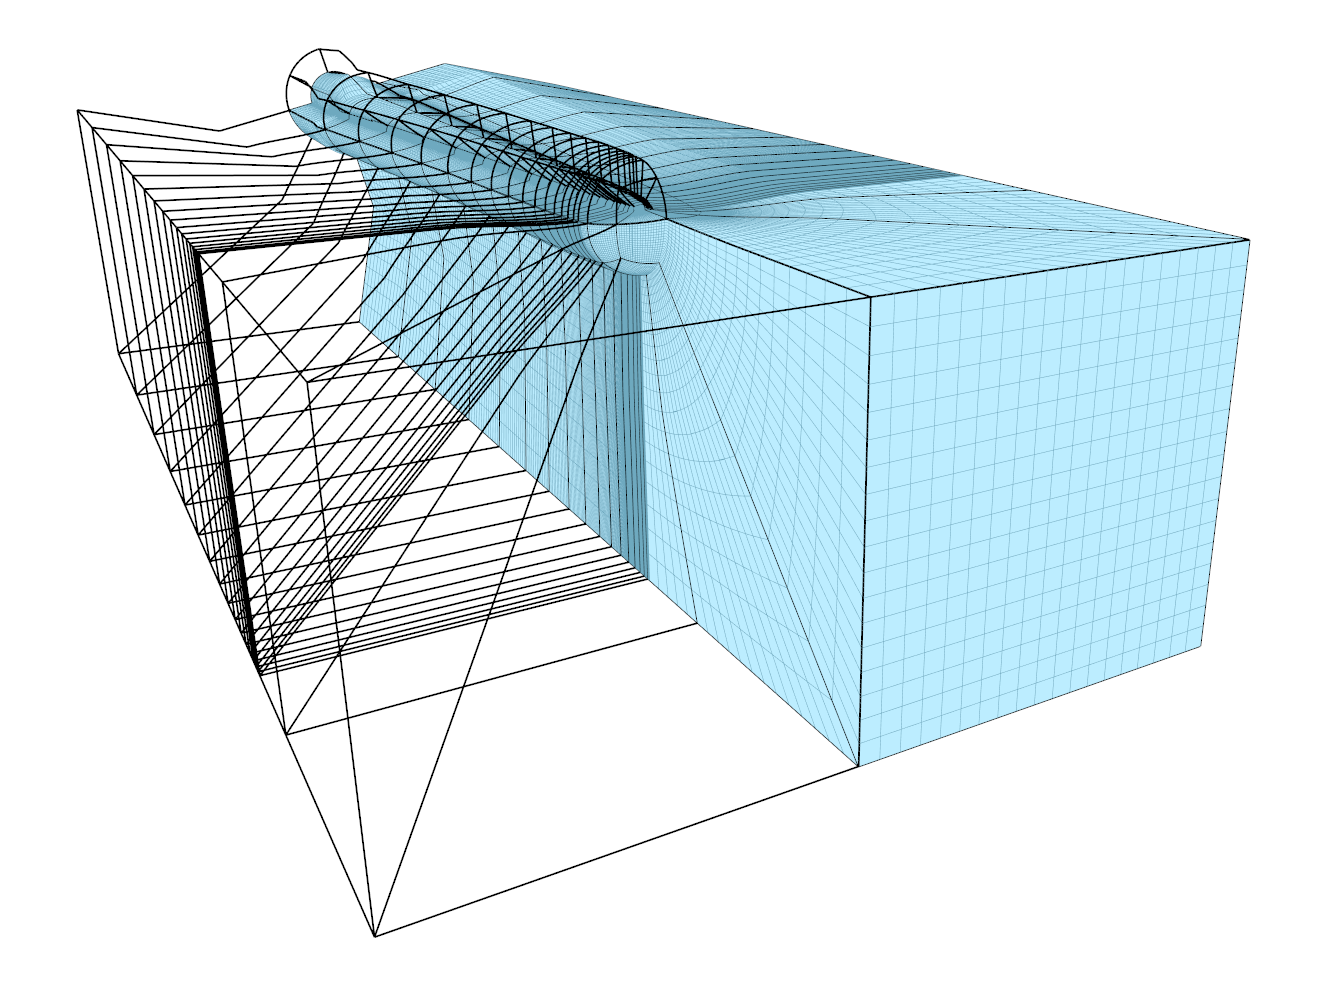
\includegraphics[width=0.3\textwidth]{figs/block-1}
  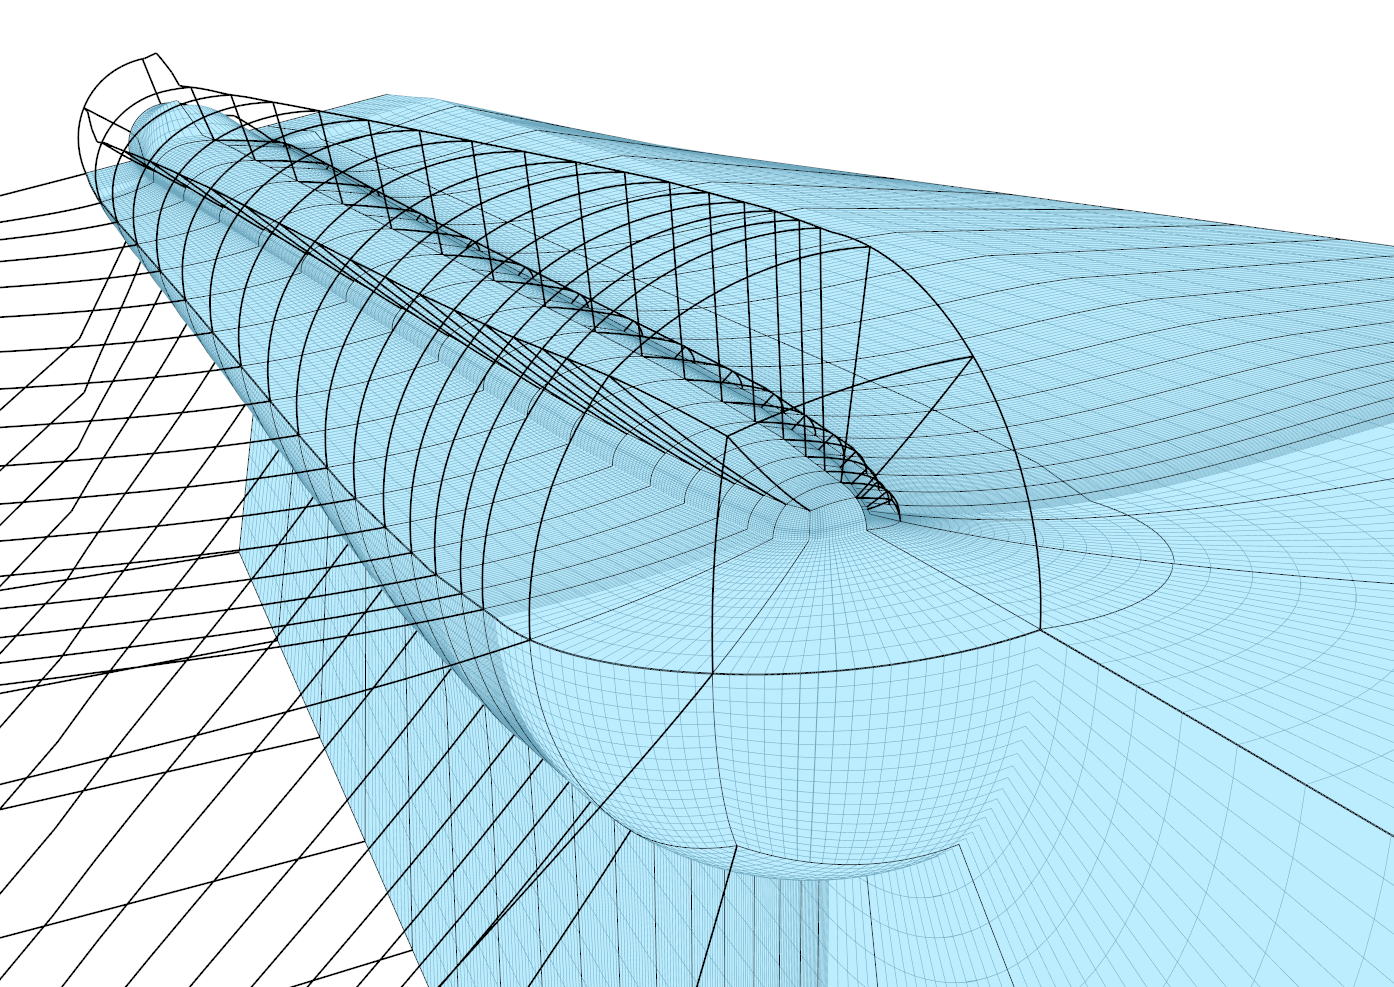
\includegraphics[width=0.3\textwidth]{figs/block-2}
  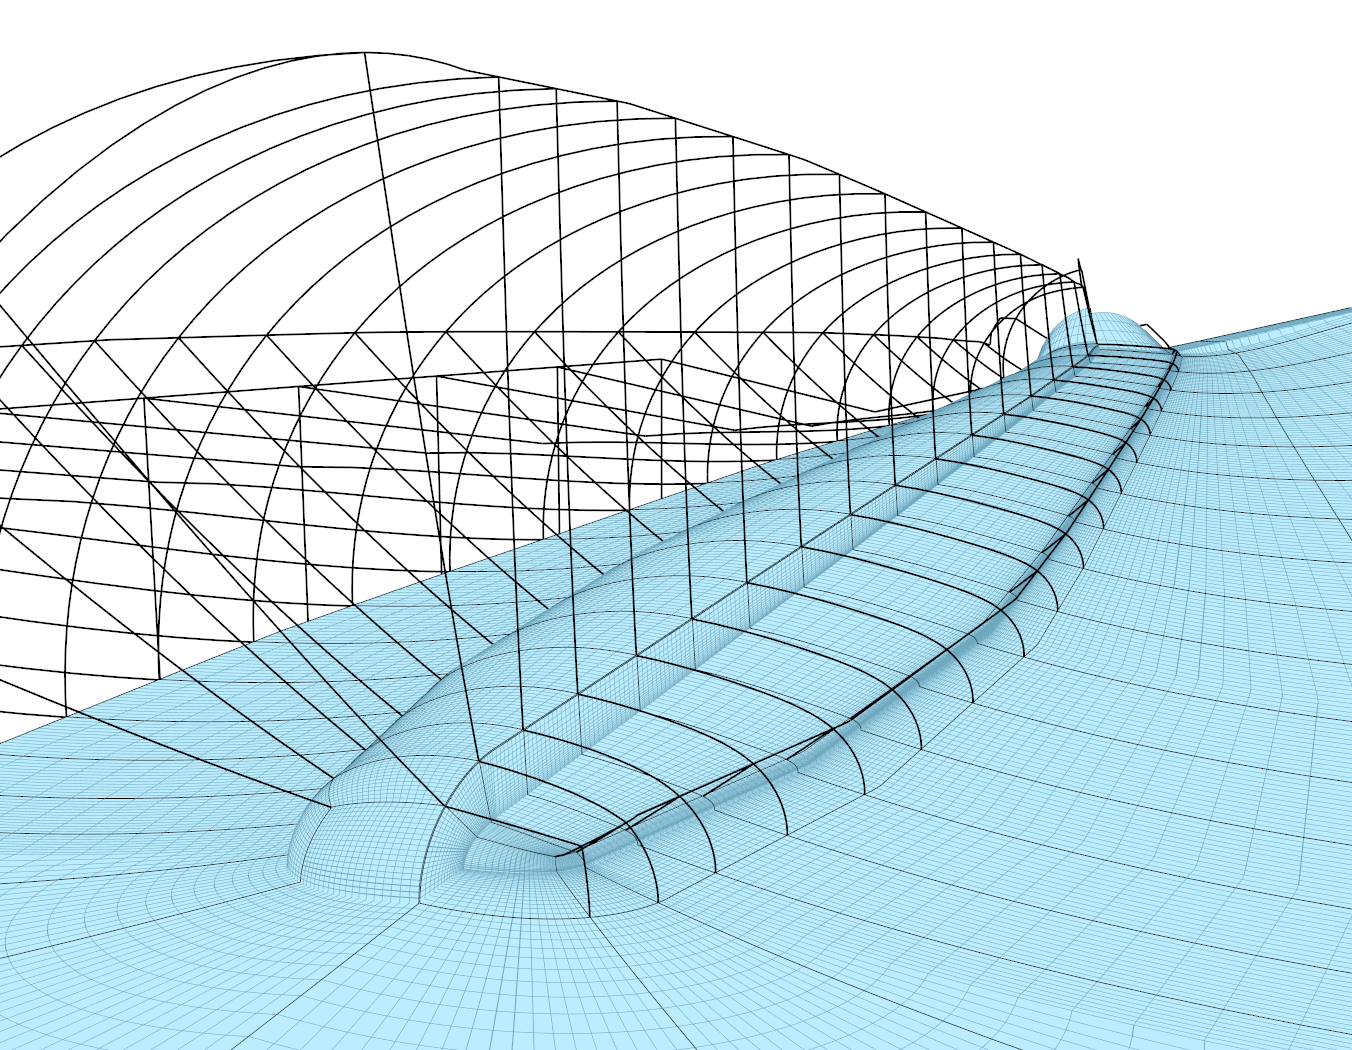
\includegraphics[width=0.3\textwidth]{figs/block-3}
  \caption{The full mesh block structure.}
  \label{fig:full}
\end{figure}

\section{Conclusion and future work}

A 2D version of the mesh generator has been developed to generate spline based
meshes for NACA0015 \cite{Nordanger2015sap} and NACA0012 \cite{Nordanger2015ict}
air foils for computation fluid dynamics studies and cylinder with an attached
bar \cite{Nordanger2015nbf} for fluid structure interaction simulations. All
these papers give detailed analyses of the mesh quality using different
criteria.

A more sophisticated 3D version of the code has been used to study thermal heat
storage in concrete. In the work thermal induced expansion and resulting
stresses were analyzed in addition to the heat storage characteristics for
different geometries. Currently a new concept based on strip theory to simulate
fluid structure interaction of a full 3D blade is being tested.

A highlight of the mesh generator is the ease of control on the mesh quality
allowed by changing key parameters like geometry, local resolution and load
balancing. The tool presented in this paper bridges a gap that existed in the
comprehensive design methodology that is being developed to conduct fluid
structure interaction simulation of a full offshore wind turbine
\cite{Rasheed2014csm}. Although the generator has been developed for our
indigenous tool IFEM it is fully compatible with other CFD tools like OpenFOAM.
The methodology ensures exact geometric representation and hexahedral elements
everywhere. The block structured meshing approach offers more flexibility in
optimal load balancing for high performance computing.

Currently, work is ongoing to handle even more complex geometries like terrain,
groups of buildings and heat exchangers with high performance computing in mind.

\section*{Acknowledgements}

The authors acknowledge the financial support from the Norwegian Research
Council and the industrial partners of the FSI-WT (216465/E20)
(\url{http://www.fsi-wt.no}) projects.

\bibliography{common/references}
\bibliographystyle{model3-num-names}

\end{document}
